\documentclass[12pt]{article}

\usepackage[utf8]{inputenc}
\usepackage[spanish,activeacute]{babel}
\usepackage{graphicx}
\usepackage{subcaption}
\usepackage[colorlinks, citecolor=black, urlcolor=black, bookmarks=false, hypertexnames=true]{hyperref} 
\usepackage{url}
\usepackage{listings}
\usepackage{color}

\definecolor{dkgreen}{rgb}{0,0.6,0}
\definecolor{gray}{rgb}{0.5,0.5,0.5}
\definecolor{mauve}{rgb}{0.58,0,0.82}

\lstset{frame=tb,
  language=HTML,
  aboveskip=3mm,
  belowskip=3mm,
  showstringspaces=false,
  columns=flexible,
  basicstyle={\small\ttfamily},
  numbers=none,
  numberstyle=\tiny\color{gray},
  keywordstyle=\color{blue},
  commentstyle=\color{dkgreen},
  stringstyle=\color{mauve},
  breaklines=true,
  breakatwhitespace=true,
  tabsize=3
}

\title{Sistemas de Recuperación de Información \\ Search Engine Optimization (SEO)}
\author{
    Samuel David Suárez Rodríguez, C512 \and
    Enmanuel Verdesia Suárez, C511
}
\date{}

\begin{document}

\maketitle

Los Motores de Búsqueda (Search Engines) son sistemas de recuperación de información, puesto que realizan búsquedas en un conjunto de datos de gran escala, específicamente sitios web, extrayendo la información relacionada acorde a una consulta.

Estos motores previamente indexan los sitios recolectando información básica de ellos, la cual incluye el URL, palabras claves, el código que estructura el sitio y los enlaces que contiene. Este proceso es realizado periódicamente pues los sitios pueden ser modificados de forma regular.

La información recolectada es almacenada en una base de datos, lo cual facilita el acceso a ella de forma más directa a la hora de responder a una consulta, dicha base de datos es conocida como el \textbf{índice del motor de búsqueda} \cite{what_is_seo}.

Todos los motores utilizan alguna métrica que permite definir la relevancia de determinado resultado con respecto a una consulta, por ejemplo, el algoritmo de Google se basa en una métrica denominada page rank \cite{pr}. Por lo que sitios con valores más altos de page rank tienden a aparecer más alto en la lista de resultados y por tanto obtienen más tráfico de usuarios.

Es aquí donde surge la necesidad de aplicar SEO. Empresas y negocios puede obtener clientes de los usuarios del motor de búsqueda, dichos clientes tienen un costo de adquisición relativamente nulo.

\section{Técnicas de SEO}
Las técnicas a continuación son utilizadas para mejorar el ranking de un sitio ante los motores de búsqueda.

\textbf{White-hat} SEO refiere al conjunto de técnicas que sigue las guías del motor de búsqueda, por tanto este no penaliza a los sitios webs que hacen su uso para obtener un mejor page rank.

Entre estas técnicas se encuentran:
\begin{itemize}
    \item[•] Escritura de contenido original con palabras claves de alta calidad.
    \item[•] Uso de meta etiquetas de HTML, etiquetas para los encabezados.
    \item[•] Enlaces en otro sitios webs que referencian al sitio así como enlaces internos que ayudan al motor de búsqueda a conocer la estructura del sitio web.
\end{itemize}

Los aplicación de estas técnicas no tiende a incrementar de manera rápida el tráfico orgánico hacia un sitio web, esto sucede de forma paulatina, y ofrece la seguridad de que el motor no penalizara el ranking del sitio en un futuro.

\textbf{Black-hat SEO} es el proceso opuesto a Black-hat SEO. Esta técnica no sigue las guías del navegador, por lo que puede obtener resultados mas eficientes en el ranking en con menor tiempo y esfuerzo, lo que puede causar que páginas con contenido de baja calidad ocupen buenos puestos en una consulta por el usuario. Pero el hecho de que esta practica viole las pautas de los motores de búsqueda, causa que en el futuro el sitio web sea penalizado y disminuya su ranking.

Entre este tipo de técnicas se incluye:

\begin{itemize}
    \item[•] Keyword stuffing.
    \item[•] Usar texto invisible al usuario en el contenido y no relacionado con el contenido del sitio para aumentar la densidad de palabras clave.
    \item[•] Granjas de enlaces, las cuales consisten en grupos de sitios los cuales se conectan unos a otros a traves de enlaces, lo cual incrementa la popularidad de estos.
    \item[•] Cloaking, conocido como spamindex, es la técnica mediante la cual se le muestra a los bots que indexan la web contenido diferente al que se muestra en la página al usuario. De esta forma un sitio especifico puede salir ante una consulta no relacionada con su contenido.
\end{itemize}

Este tipo de acciones son perseguidas por los motores de búsqueda y detectadas con diferentes algoritmos. Si un sitio web es detectado como fraudolento, es penalizado en el ranking e incluso puede ser removido del indice.

\textbf{Gray-hat} se encuentra en medio de los conjuntos anteriores, de tal manera son técnicas que pueden no crear mucho impacto en el ranking del sitio y aun asi estar bajo riesgo de penalización.

\section{Ejemplo de Optimizaciones}
Mostraremos interés en técnicas White-hat pues estas a pesar de tomar mas tiempo en ofrecer resultados, lo hacen de forma solida y mas segura para el sitio.

Existen dos tipos de SEO, \textbf{On Page SEO} y \textbf{Off Page SEO}, las primeras son modificaciones que pueden ser realizadas directamente al código y el contenido del sitio web, la segunda se refiere a acciones que pueden ser tomadas desde fuentes externas y que pueden mejorar el posicionamiento del sitio.

\subsection{On Page SEO}

\begin{itemize}
\item \textbf{Contenido}

Entre el 65\% - 75\% del contenido de la página web debe ser único y de alta calidad, además, la relación entre texto y HTML debe estar entre 25\% - 75\%. Los crawlers de los motores de búsqueda visitan el sitio y crean una copia del contenido en su base de datos, si encuentran otra página web con el mismo contenido, entonces esta es penalizada.

\item \textbf{Investigación de palabras claves}

A día de hoy motores de búsqueda como Google, no dan atención extra a palabras claves, por tanto investigar cuales son las palabras claves correctas puede ser una tarea importante al crear un sitio web. Una buena palabra clave debe coincidir con el contenido de la página.

\item \textbf{Etiqueta} \verb+title+

Los títulos de las diferentes páginas de un sitio web deben ser únicos y precisos, de tal forma que describan el contenido de la página de forma breve.

Ejemplo:
\begin{lstlisting}
<html>
<head>
    <title>Brandon's Baseball Cards - Buy Cards, Baseball News, Card Prices</title>
</head>
<body>
...
\end{lstlisting}

\item \textbf{Etiquetas} \verb+alt+

La etiqueta \verb+alt+ es de gran importancia pues esta describe al motor de búsqueda el contenido detrás de una imagen. Este es el texto que aparece cuando se mueve el cursor sobre una imagen en el navegador. También son usadas por los lectores de pantalla para mejorar la accesibilidad.

Ejemplo:
\begin{lstlisting}
<img title="Imagen" src="image.jpg" alt="An octocat coding"/>    
\end{lstlisting}

\item \textbf{Etiquetas de metadatos (}\verb+meta+\textbf{)}

Estas definen metadatos del sitio y su principal objetivo es ser procesadas por los motores de búsqueda, por ello se recomienda describir en estas que tipo de contenido presenta la página y ofrecer toda la información adicional posible.

Es recomendado poner una descripción que se encuentre entre 70 - 160 caracteres, palabras claves, autor, etc.

Debe asegurarse que todas las páginas del sitio posean esta información.

Ejemplo:
\begin{lstlisting}
<head>
    <meta charset="UTF-8">
    <title>Brandon's Baseball Cards - Buy Cards, Baseball News, Card Prices</title>
    <meta name="description" content="Brandon's Baseball Cards provides a large selection of vintage and modern baseball cards for sale. We also offer daily baseball news and events.">
    <meta name="author" content="John Doe">
    <meta name="viewport" content="width=device-width, initial-scale=1.0">
</head>
\end{lstlisting}

\item \textbf{Etiquetas} \verb+meta+  \textbf{para robots} \cite{meta_robots}

Esta etiqueta indica como debe ser indexada y servida a los usuarios en una consulta determinada página. Permite controlar que contenido se indexa y cual no en un sitio web.

Ejemplo:
\begin{lstlisting}
<head>
    <meta name="robots" content="noindex"/>
    (...)
</head>
\end{lstlisting}

\item \textbf{Datos estructurados} \cite{rich_results}

Google usa estos datos para comprender mejor el contenido de una página. Cuando se muestran resultados a una búsqueda estos datos se usan para ofrecer información adicional, lo que puede atraer más tráfico al sitio.

Por ejemplo, si se tiene un e-commerce cada producto puede tener como datos estructurados la calificación cantidad de comentarios, el precio, etc. A la hora del motor de búsqueda responder a una consulta con con uno de los productos, estos datos son utilizados para enriquecer el resultado.

Como punto adicional, estos tienen mayor relevancia en las consultas realizadas pues los usuarios pues pueden buscar productos por estos parámetros.

\item \verb+https+ \textbf{por encima} \verb+http+

Los motores de búsqueda exhortan a los sitios a usar \verb+https+ dado que ofrece más seguridad a los usuarios que acceden a los sitios.

\item \textbf{Enlaces internos}

Estos enlaces facilitan la comprensión de la estructura del sitio web para los motores de búsqueda, sirven de puente para visitar cada una de las páginas de un sitio web.

Ejemplo:
\begin{lstlisting}
<a href="http://www.same-domain.com/" title="Keyword Text">Keyword Text</a>    
\end{lstlisting}

En ocasiones es recomendable que se indiquen enlaces con el parámetro \verb+rel=nofollow+, de tal forma que los motores no procesen el contenido que tienen. Por ejemplo, sucede cuando estos enlaces llevan a contenido (no confiable) compartido por los usuario y que puede reflejar la mala calidad en el sitio.

\item \textbf{Mapas del sitio} \cite{sitemaps}

A pesar de que un sitio web puede ser rastreado e indexado sin usar sitemaps y usar uno no mejora la posición en el ranking, este hace mas sencillo para los motores indexar el sitio. Es recomendado para indexar páginas que hayan quedado fuera de los enlaces internos del sitio o que sean difíciles de encontrar. Ademas permiten encontrar información importante sobre imágenes y videos que es inaccesible a los crawlers.

Example:
\lstset{language=XML}
\begin{lstlisting}
<?xml version="1.0" encoding="UTF-8">
<urlset xmlns="http://www.sitemaps.org/schemas/sitemap/0.9" xmlns:image="http://www.google.com/schemas/sitemap-image/1.1">
    <url>
        <loc>http://www.example.com/sample-page</loc>
        <image:image>
            <image:loc>http://www.example.com/image.jpg</image:loc>
        </image:image>
        <image:image>
            <image:loc:>http://www.exampe.com/image2.jpg</image:loc>
        </image:image>
    </url>
</urlset>
\end{lstlisting}

\item \textbf{Optimizar el sitio para dispositivos móviles} \cite{mobile}

Especifícamente en el año 2016 Google anunció que iba a priorizar la indexación del contenido que ofrecen los sitios a los dispositivos móviles.

Esto quiere decir que si los sitios no están correctamente diseñados para ofrecer esta funcionalidad, muestran menos contenido o de baja calidad en ella, probablemente resulten penalizados.

Motivo de esto es que la gran mayoría de los usuarios realizan las consultas desde sus dispositivos móviles.


\end{itemize}

\subsection{Off Page SEO}
\begin{itemize}
\item \textbf{Backlinks}

Estos son los enlaces en otros sitios webs que apuntan al sitio de interés, los cuales permiten determinar al motor de búsqueda determinar si el sitio es relevante o no.

Que un sitio web tenga más backlinks que otro no significa que este último vaya a posicionarse por debajo en el ranking pues si los enlaces de este son de mayor calidad puede ser mas relevante para el ranking \cite{imp_seo}.

\item \textbf{Redes sociales}

Las redes sociales juegan un papel vital a la hora de traer nuevos visitantes a sitios webs, además muchas de ellas soportan "follow links" los cuales generan backlinks de alta calidad.

\item \textbf{Búsqueda local}

Google con el algoritmo Pigeon hizo énfasis en ofrecer a los usuarios resultados de acuerdo a su ubicación geográfica, lo cual puede ser explotado de forma positiva por los sitios webs en una localidad.

\item \textbf{Herramientas de webmaster}

Estas son herramientas que permiten identificar problemas y errores en sitios webs, además pueden decir cómo, quién, cuándo y desde dónde el visitante interactúa con el sitio web.

\end{itemize}

\section{Algoritmos de Google}

Como ya hemos visto, el principal objetivo de las técnicas de SEO es mantener el sitio de acuerdo a los lineamientos de los motores de búsqueda para obtener un mejor posicionamiento en el ranking de resultados.

Un sitio puede estar bien posicionado en este ranking por mucho tiempo, pero los algoritmos también sufren cambios o actualizaciones que pueden causar de un momento a otro obtener una Página de Resultados del Motor de Búsqueda (SERP, según sus siglas en inglés) totalmente diferente.

Una vez esto sucede, los sitios deben ajustarse al nuevo cambio y seguir las mejores prácticas para subir en el ranking de acuerdo a los nuevos requerimientos.

Vale la pena destacar que Google es el principal motor de búsqueda de acuerdo a la cantidad de usuarios, por tanto los sitios deben mostrar especial interés en él.

\begin{figure}[!h]
    \centering
    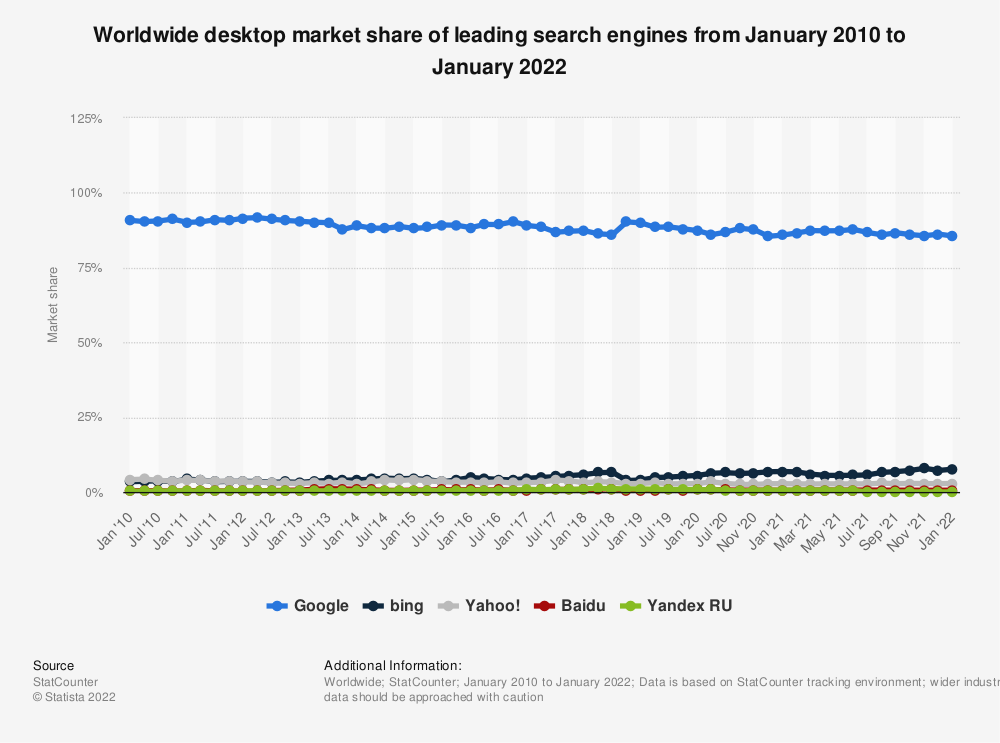
\includegraphics[width=\linewidth]{images/216573.png}
  \end{figure}
\subsection{Actualizaciones}

\begin{itemize}

\item \textbf{Panda [febrero del 2011]:} La actualización estuvo diseñada para reducir la posición de sitios de poco valor para los usuarios, que copian contenido, etc. A la misma vez favoreció mejor posicionamiento para sitios de alta calidad con contenido original e información como investigaciones, reportes, análisis, etc. \cite{panda}

\item \textbf{Penguin:} Esta algoritmo fue una extensión a Panda, pues después de la aplicación de aquella aun quedaban muchos sitios ganando posicionamiento a través de técnicas black-hat. Principalmente el spam de enlaces y prácticas manipulativas de este tipo. Ha recibido múltiples actualizaciones a lo largo de los años. \cite{penguin}

\item \textbf{Page Layout Algorithm [enero del 2012]:} Estuvo enfocado en penalizar sitios que con muchos anuncios estáticos, los cuales obligaran al usuario a desplazarse por la página para poder acceder al contenido.

\item \textbf{Exact Match Domain (EMD) [2012]:} Estuvo enfocada en disminuir el posicionamiento de sitios con poco contenido pero que tuviesen palabras claves en su nombre de dominio, palabras que podían coincidir con una consulta de un usuario.

\item \textbf{Hummingbird [septiembre del 2013]:} A partir de la aplicación de este se ve la búsqueda como consultas de forma semántica, en lugar de solo texto. Ahora el motor de búsqueda trata de entender el significado de la consulta en lugar de hacer match con las palabras que esta contiene y el contenido de los sitios; usa ese significado para calificar la relevancia de estos.

\item \textbf{Pigeon [julio del 2014]:} Benefició principalmente a negocios locales, pues Google comenzó a mostrar resultados en las búsquedas de acuerdo a la localización de los usuarios. Esta actualización mejoró la experiencia de los usuarios y se vio el impacto con un incremento en el tráfico de los sitios beneficiados.

\item \textbf{Mobilegeddon [abril del 2015]:} Esta actualización estuvo enfocada en optimizar la experiencia para móviles. \cite{mobilgeddon}

\item \textbf{RankBrain [octubre del 2015]:} RankBrain es un sistema de aprendizaje de máquina que permite entender mejor las consultas. A partir de la aplicación de este se empezó a ver los elementos en las consultas como entidades y crear relaciones entre ellas. Así Google podía analizar consultas no vistas previamente de forma textual y relacionarlas con consultas similares.

\item \textbf{Intersticiales Intrusivos [agosto del 2016]:} Los sitios que muestran pop-ups que ocupan el contenido y es necesario cerrarlos para continuar leyendo fueron los principales afectados por esta actualización. De igual forma ocurre si es necesario pasar por uno para acceder al contenido.

\item \textbf{Mobilegeddon 2.0 [marzo del 2016]}: Siguiendo las pautas de la anterior se daría un impulso aun mayor a los sitios optimizados a dispositivos móviles. \cite{mobilgeddon2}

\item \textbf{Fred [mayo del 2017]:} Esta actualización estuvo enfocada en penalizar sitios percibidos como resultados de baja calidad, ya sea por tener poco contenido o por mostrar demasiados anuncios. Muchos sitios fueron afectados pore sta actualización, algunos vieron su tráfico disminuir un 50 - 90\%. \cite{fred}

\end{itemize}

Han ocurrido más actualizaciones no mencionadas en esta lista, además algunas de ellas no son anunciadas públicamente pues Google no es del todo transparente respecto a los cambios en sus algoritmos.

\section{Conclusiones}

Se ha podido apreciar a lo largo de este reporte que el objetivo de los motores de búsqueda es ofrecer la mejor experiencia y contenido posible a los usuarios ante una consulta. En este sentido fuerzan a los sitios webs a mantener prácticas que no vayan en decremento de la calidad del contenido en la web.

De forma mutua los sitios tratan de cumplir con los requerimientos pues millones de usuarios que usan motores de búsqueda como Google, Bing, DuckDuckGo, etc. son potenciales clientes o usuarios de ellos, pero esto solo es posible si se logra aparecer en los primeros resultados de las SERP.

Además no es suficiente con implementar buenas prácticas, los webmasters deben estar atentos a cambios en los algoritmos, que ante una actualización, pueden cambiar el posicionamiento de un sitio de forma inesperada.

\bibliography{bib} 
\bibliographystyle{ieeetr}

\end{document}